\section{Ancora amplificatore invertente}
In questa sezione si vuole misurare la frequenza di taglio e lo slow rate del amplificatore così costruito.
\subsection{Risposta in frequenza}
Qui si vuole vedere il comportamento del OpAmp come circuito a un polo, dunque se ne vuole misurare la risposta in frequenza trovando una frequenza di taglio e un attenuazione $\SI{-20}{dB/\deca}$ tipica dei passa-basso.
%Per far questo si è scelto di campionare le frequenze in un range da $\SI{0.2}{\Hz}$ a $\SI{1}{\MHz}$.
L'ampiezza dell'ingresso, per risparmiare tempo, si è tenuta costante a $\SI{1.04}{V}$. Quest'ultima scelta ha impedito di aumentare la frequenza oltre $\SI{1}{\MHz}$ per mantenere le pendenze massime delle sinusoidi al di sotto della pendenza di slewrate(da datasheet $13 MVs^{-1}$).%affermazione da verificare...
I dati sono stati fittati con due rette (una retta affine, 2 parametri, una retta costante, 1 parametro), senza considerare gli errori di calibrazione degli strumenti, ne l'errore sulla tensione di ingresso. I cut-off sulle frequenze scelti per separare la regione in cui l'amplificazione è costante e la regione in cui l'amplificazione scende a circa $-20dB/decade$ sono poste a $\SI{40}{\kHz}$ e $\SI{400}{\kHz}$. I dati e i fit sono riassunti in figura \ref{f:BODE2}

\begin{figure}[h]
	\centering
	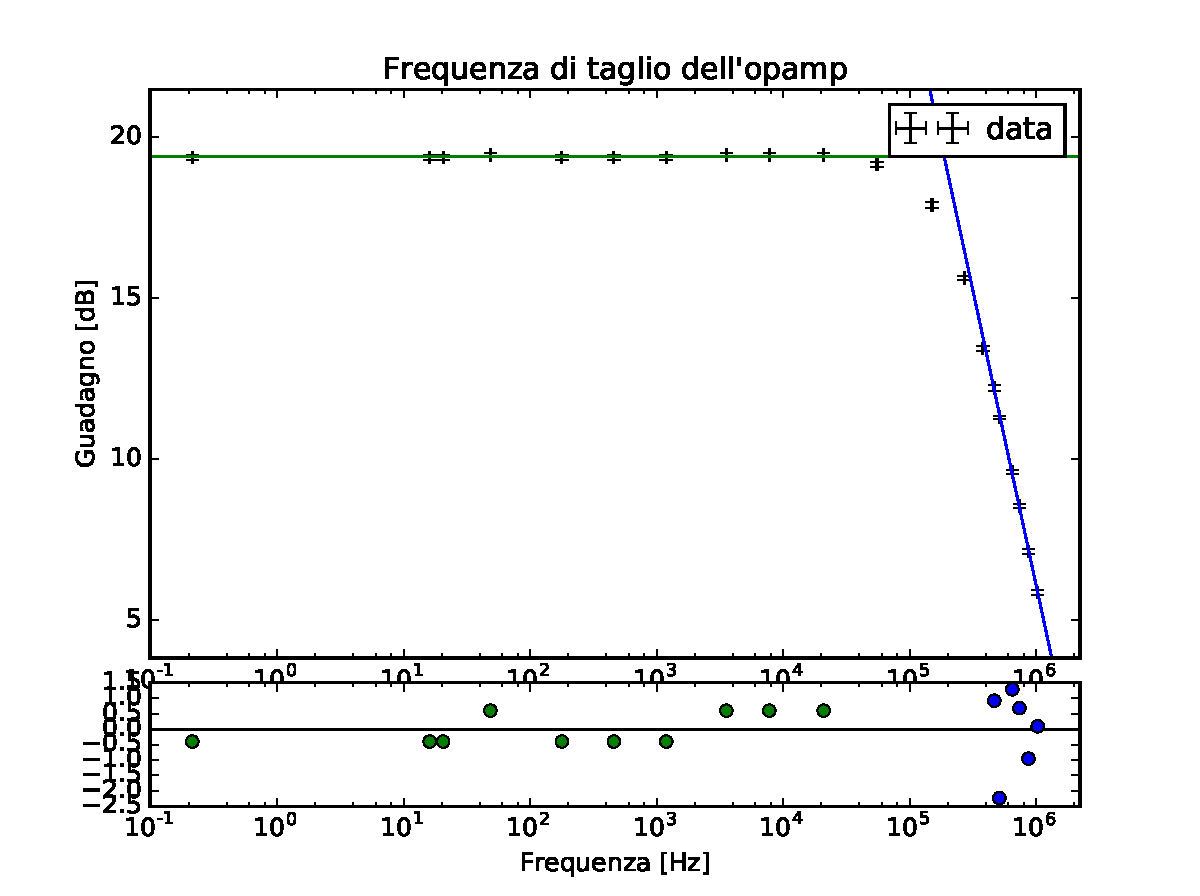
\includegraphics[scale=0.6]{fig2bode.pdf}
	\caption{Plot di bode di dati e fit}
	\label{f:BODE2}
\end{figure}

Per la retta si sono ottenuti i seguenti parametri:\\
$q =\chi^2{19.41 \pm 0.02}{dB}$\\
$\chi^2 = 2.40$ ($9$ DoF, $p = 0.98$)\\

Questo farebbe pensare a una sovrastima degli errori di lettura. In effetti per molti dati il segnale letto è uguale all'interno dell'errore di lettura.
A questi dati grezzi va aggiunto l'errore di calibrazione e l'errore sulla tensione in ingresso. 
Dati $\sigma_l$ l'errore su $q$ dato dagli errori di lettura, $\sigma_c$ l'errore su $V_{out}$ dovuto alla calibrazione dell'oscilloscopio e $\sigma_{in}$ l'errore totale sulla tensione in ingresso, si ottiene (propagando in quadratura e considerando indipendenti le fonti di errore, utilizzando come errore di calibrazione sulle misure dell'oscilloscopio il $3\%$ del valore misurato):
$\sigma_q^2=\sigma_l^2+400(\frac{\sigma_{in}^2}{V_in}+\frac{\sigma_c^2}{V_{out}^2})$\\
Inserendo i dati si ottiene:\\
$\sigma_q=0.84$\\
Dunque $q=19.41\pm 0.84$, compatibile con quanto atteso per il guadagno in continua.\\
Per la retta obliqua si ottiene invece:\\
$m =\SI{-18.32 \pm 0.37}{ dB/\deca}$\\
$q = 116.0 \pm 2.2 dB$\\
$cov=-0.998$
$\chi^2 =2.19$ ($4$ DoF,$ p = 0.70$)\\

Anche qui vanno aggiunti gli errori di calibrazione sulle tensioni di ingresso e uscita. 
Per quanto riguarda $q$ la correzione da apportare è la stessa, dunque si ottiene un valore di:\\
$q=116.0 \pm 2.3 dB$\\
Per quanto riguarda $m$ si è stimato di calibrazione sul rapporto incrementale di due punti presi a caso con gli errori di calibrazione. Si è ottenuto:
$m=\SI{-18.3 \pm 1.8}{ dB/\deca}$

Con questi dati si può stimare la frequenza di taglio come la frequenza di intersezione delle due rette:\\
$f_t=\SI{187.070\pm 0.08}{\kHz}$ %oppure pm 93470.9 se si usano gli errori con le calibrazioni corretti!!!!!

\subsection{Slew-rate}
In questa sezione lo scopo è misurare lo slew-rate del componente. Per fare questo ci si è inviata in ingresso un onda quadra di ampiezza $1.04 V$ e frequenza $\SI{1}{\kHz}$. Si è ottenuto il comportamento mostrato in figura \ref{f:SLWRT}. Esso a prima vista sembra compatibile con il normale comportamento di un circuito ad un polo sotto un segnale a scalino % ed infatti probabilmente lo è...
\begin{figure}[h]
	\centering
	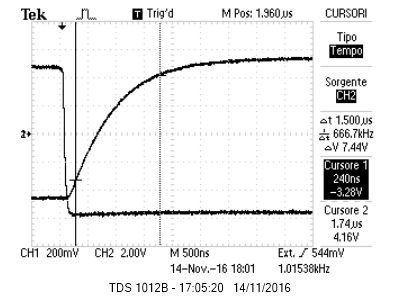
\includegraphics[scale=0.6]{slewrate.png}
	\caption{Output dell'onda quadra}
	\label{f:SLWRT}
\end{figure}

ma, nonostante tutto, nella prima parte della salita \ref{f:EXPD} si può notare uno scostamento dalla natura esponenziale aspettata.\footnote{In effetti con una misura più accurata in laboratorio si sarebbe potuto evitare un analisi dati così complessa}
%\footnote{Il vero scopo è fare vedere che con abbastanza sbatta si riesce a far tornare tutto in tempo di analisi dati, ma che palle!!! Potevamo prendere i dati come dio comanda}
Per discernere il tratto in cui lo slow-rate si fa sentire dal normale comportamento da passa-basso si sono fittati i dati con una curva esponenziale del tipo $V_{out}=V_a-V_be^{-t/\tau}$ \ref{f:EXP} (acquisiti al computer tramite l'oscilloscopio) con un cut-off inferiore sui tempi mobile \ref{f:EXPD}(il componente inizia la salita  $\SI{1.5e-7}{s}$ dopo il triggering, si è spostato il punto di cut-off in una finestra tra $\SI{1.5e-7}{s}$ a $\SI{3.0e-7}{s}$) Si è dunque plottata il p-value in funzione del punto di cut-off \ref{f:MAD}.

\begin{figure}[h]
	\centering
	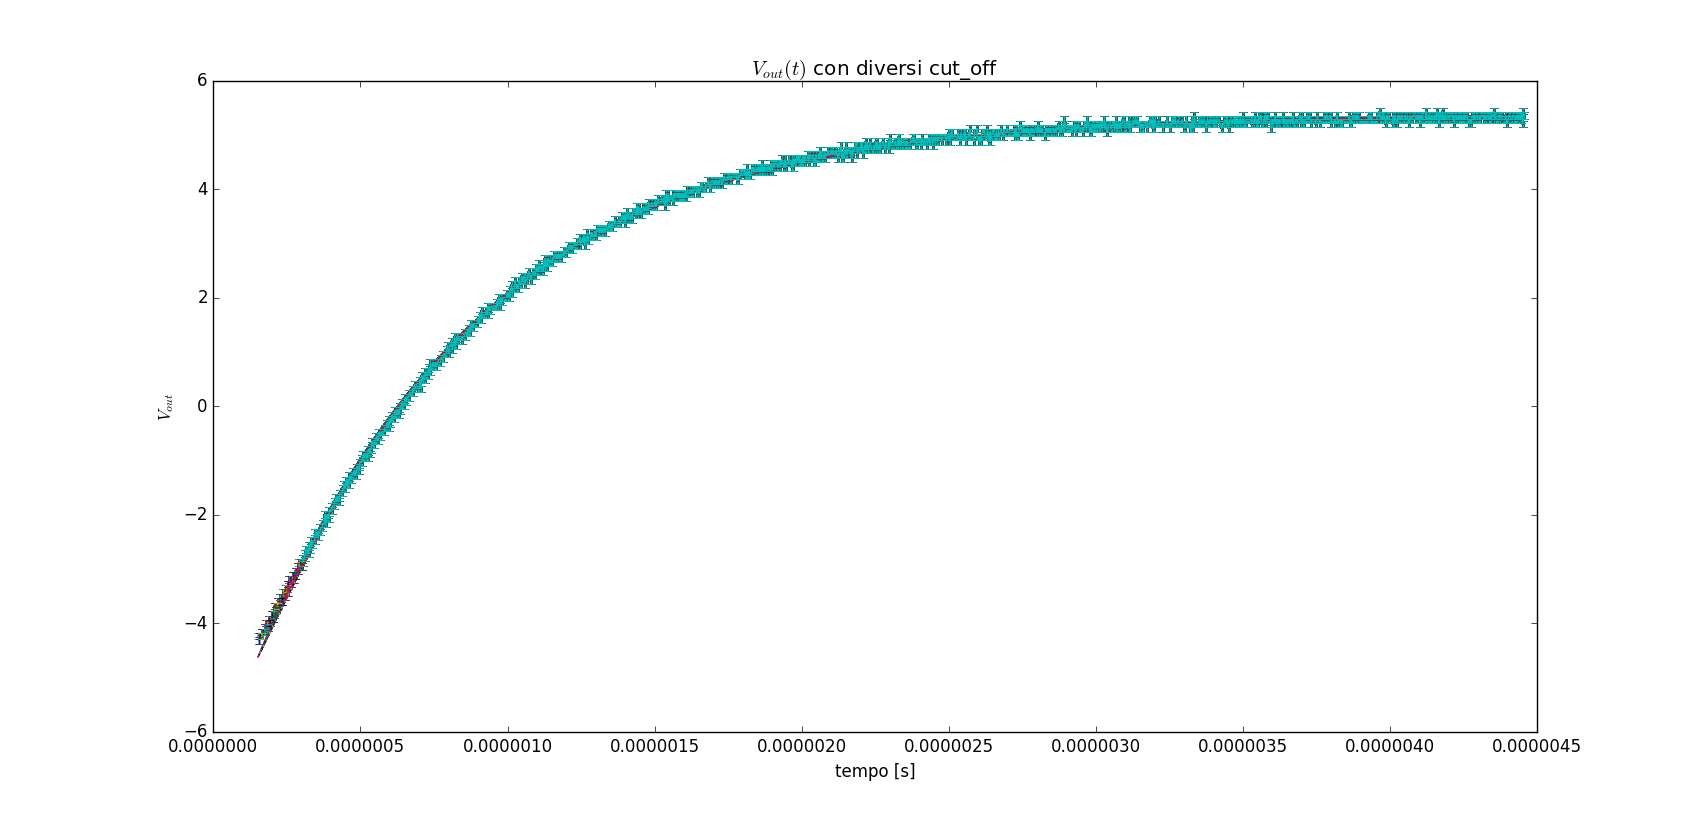
\includegraphics[scale=0.4]{esponenziali.png}     %è messo png apposta, altimenti è troppo pesante
	\caption{Output dell'onda quadra, fittato con cut-off variabili}
	\label{f:EXP}
\end{figure}

\begin{figure}[h]
	\centering
	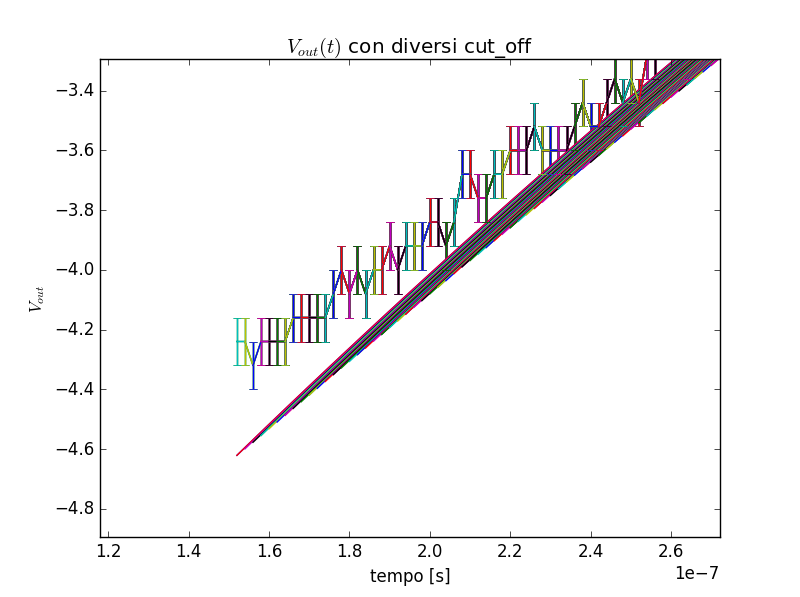
\includegraphics[scale=0.6]{coda_exp.png}
	\caption{Dettaglio dei fit, nella zona di interesse}
	\label{f:EXPD}
\end{figure}

\begin{figure}[h]
	\centering
	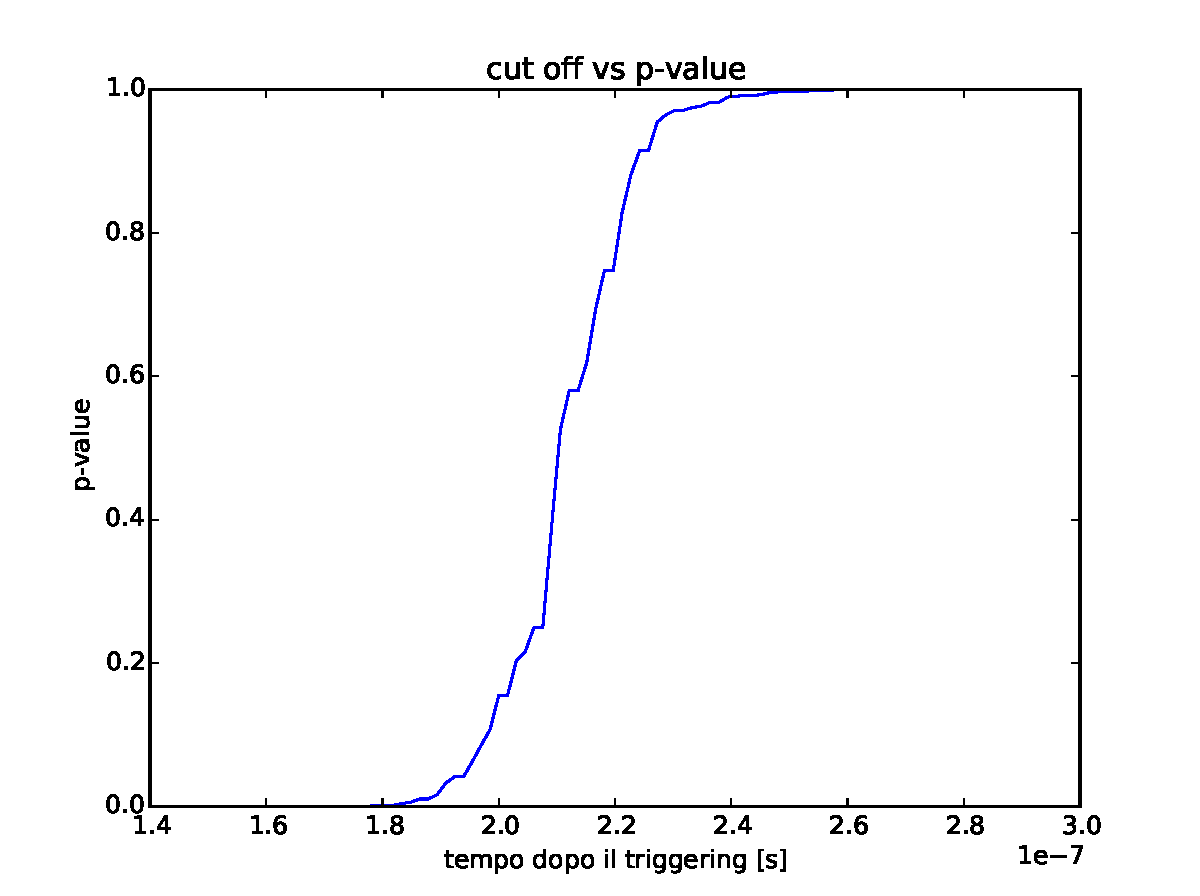
\includegraphics[scale=0.6]{madness.pdf}
	\caption{P-value in funzione del cut-off}
	\label{f:MAD}
\end{figure}

Le cose notevoli sono:\\
-La probabilità va a 1, dunque gli errori sono evidentemente sovrastimati\\
-Nonostante ciò, la probabilità scende a zero se si considerano dati troppo vicini a $\SI{1.5e-7}{s}$.\\
Per fittare la retta che dovrebbe dare il nostro slow-rate si è deciso di prendere il valore del cut-off per il quale la probabilità di ottenere un $\chi^2$ così elevato fittando giustamente con un esponenziale sia del $0.5 \%$, ovvero un tempo finale di $\SI{1.97e-7}{s}$ dopo il triggering.\\
In questa finestra di tempi si è dunque fatto un fit alla retta affine $V_{out}=At+B$ dove il parametro $A$ dovrebbe essere proprio lo slew-rate.
Con il fit in figura \ref{f:RETTA} (retta affine) si sono ottenuti i seguenti dati:\\
$SR={8.56 \pm 0.67}{MV/s}$\\
$B={-5.60\pm 0.11}{V}$ intercetta, parametro inutile\\
$corr=-0.99$\\
$\chi^2=8.8$ ($22$ Dof $p=0.994$)\\

Si noti che anche qui si ha un valore di $\chi^2$ troppo elevato, forse causato dalla sovrastima dell'errore di digitalizzazione. Il parametro risulta comunque non in disaccordo con il valore di riferimento $13 MV/s$, da datasheet come valore tipico.



\begin{figure}[h]
	\centering
	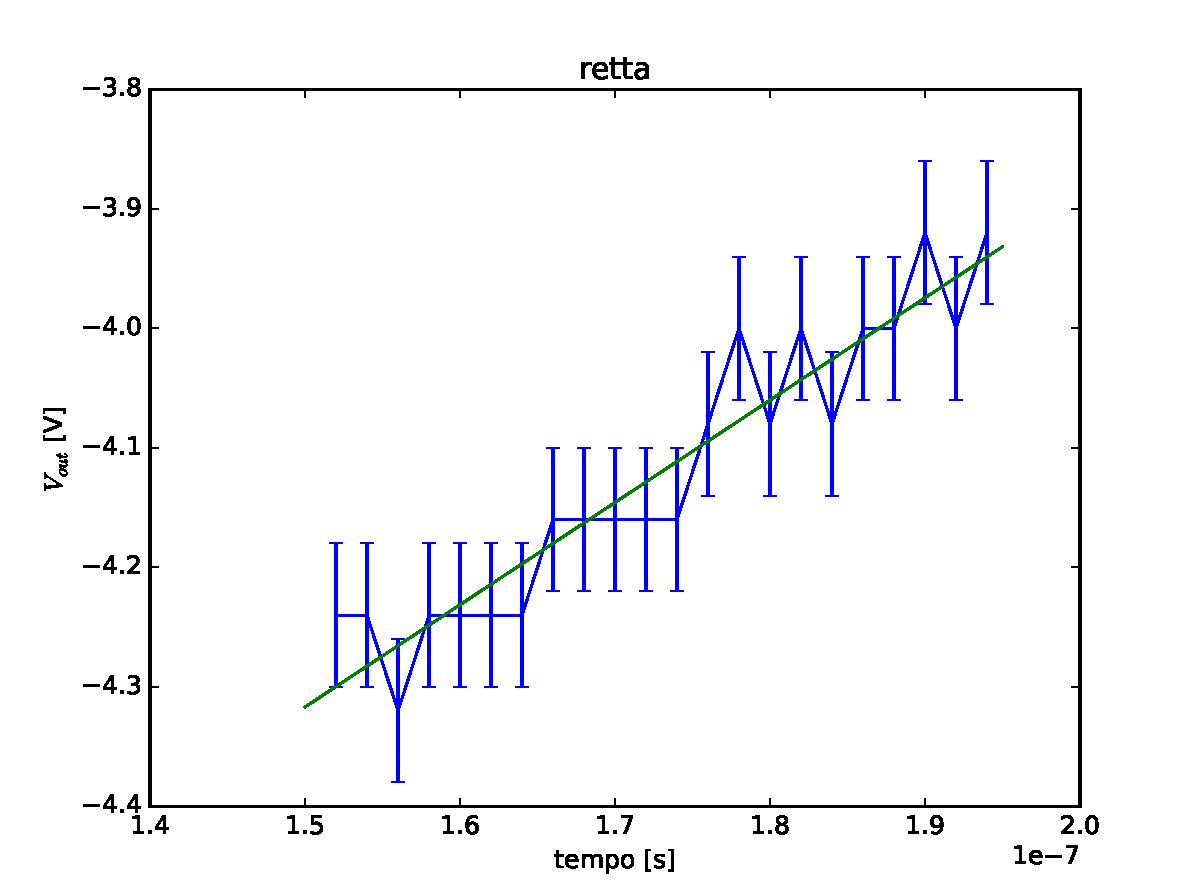
\includegraphics[scale=0.6]{retta.pdf}
	\caption{Fit dello slow-rate}
	\label{f:RETTA}
\end{figure}


\section{Amplificatore non invertente}

In questa sezione si studia il comportamento dell'amplificatore non invertente, in particolare si verifica che variando il valore dell'amplificazione (modificando la resistenza del trimmer) la banda passante verifica la ben nota formula $Af_t=cost$.\\
Il circuito è stato montato con una resistenza $R_1=\SI{214\pm 3}{\ohm}$. La tensione di ingresso si è mantenuta sempre  $V_{in}=\SI{1.04\pm 0.03}{V}$ picco-picco.
Per stimare la frequenza di taglio si è usato il metodo dei $-3dB$. Per dare una stima dell'errore sulla frequenza si è variata la stessa fin quando l'output era compatibile con l'attenuazione richiesta. Si sono inoltre misurate le resistenze del trimmer per ogni misura. \\
I dati ottenuti, riassunti in figura \ref{f:GBW}, con il risultato:
$Af_H=\SI{2.11\pm 0.05}{\MHz}$

\begin{figure}[h]
	\centering
	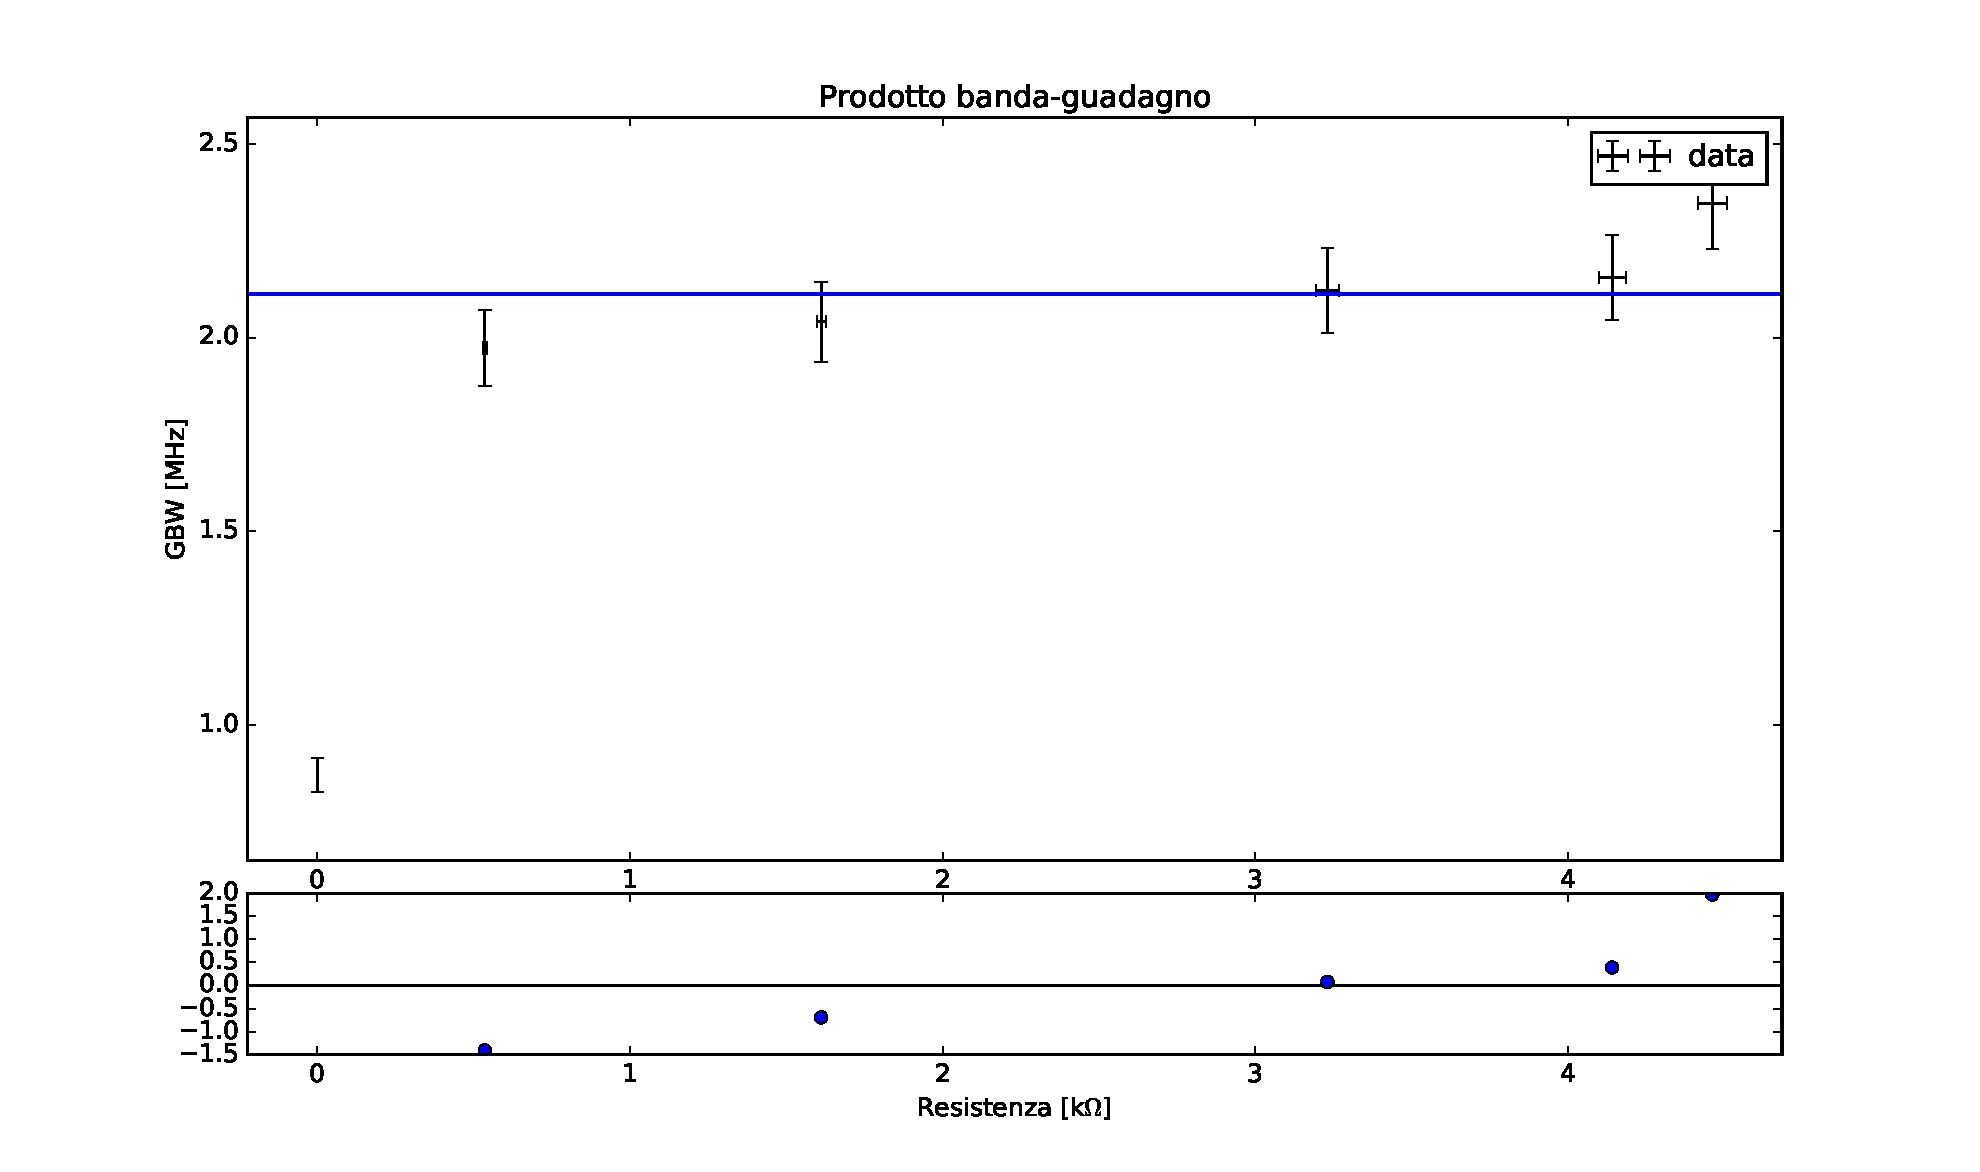
\includegraphics[scale=0.6]{GBW.pdf}
	\caption{Prodotto banda-guadagno per diversi valori della resistenza del trimmer}
	\label{f:GBW}
\end{figure}





